
\documentclass[10pt]{beamer}
\usepackage{amsmath}
\usepackage{mathtools}
\usepackage{multimedia}
\usepackage{hyperref}


\usefonttheme{professionalfonts} % using non standard fonts for beamer
\usefonttheme{serif} % default family is serif
%\documentclass[12pt]{beamerthemeSam.sty}
\usepackage{epsf}
%\usepackage{pstricks}
%\usepackage[orientation=portrait,size=A4]{beamerposter}
\geometry{paperwidth=160mm,paperheight=120mm}
%DT favorite definitions
\def\LL{\left\langle}	% left angle bracket
\def\RR{\right\rangle}	% right angle bracket
\def\LP{\left(}		% left parenthesis
\def\RP{\right)}	% right parenthesis
\def\LB{\left\{}	% left curly bracket
\def\RB{\right\}}	% right curly bracket
\def\PAR#1#2{ {{\partial #1}\over{\partial #2}} }
\def\PARTWO#1#2{ {{\partial^2 #1}\over{\partial #2}^2} }
\def\PARTWOMIX#1#2#3{ {{\partial^2 #1}\over{\partial #2 \partial #3}} }

\def\rightpartial{{\overrightarrow\partial}}
\def\leftpartial{{\overleftarrow\partial}}
\def\diffpartial{\buildrel\leftrightarrow\over\partial}

\def\BS{\bigskip}
\def\BC{\begin{center}}
\def\EC{\end{center}}
\def\BN{\begin{enumerate}}
\def\EN{\end{enumerate}}
\def\BI{\begin{itemize}}
\def\EI{\end{itemize}}
\def\BE{\begin{displaymath}}
\def\EE{\end{displaymath}}
\def\BEA{\begin{eqnarray*}}
\def\EEA{\end{eqnarray*}}
\def\BNEA{\begin{eqnarray}}
\def\ENEA{\end{eqnarray}}
\def\EL{\nonumber\\}

\newcommand{\etal}{{\it et al.}}
\newcommand{\gbeta}{6/g^2}
\newcommand{\la}[1]{\label{#1}}
\newcommand{\ie}{{\em i.e.\ }}
\newcommand{\eg}{{\em e.\,g.\ }}
\newcommand{\cf}{cf.\ }
\newcommand{\etc}{etc.\ }
\newcommand{\atantwo}{{\rm atan2}}
\newcommand{\Tr}{{\rm Tr}}
\newcommand{\dt}{\Delta t}
\newcommand{\op}{{\cal O}}
\newcommand{\msbar}{{\overline{\rm MS}}}
\def\chpt{\raise0.4ex\hbox{$\chi$}PT}
\def\schpt{S\raise0.4ex\hbox{$\chi$}PT}
\def\MeV{{\rm Me\!V}}
\def\GeV{{\rm Ge\!V}}

%AB: my color definitions
%\definecolor{mygarnet}{rgb}{0.445,0.184,0.215}
%\definecolor{mygold}{rgb}{0.848,0.848,0.098}
%\definecolor{myg2g}{rgb}{0.647,0.316,0.157}
\definecolor{A}{rgb}{1.0,0.3,0.3}
\definecolor{B}{rgb}{0.0,1.0,0.0}
\definecolor{C}{rgb}{1.0,1.0,0.0}
\definecolor{D}{rgb}{0.5,0.5,1.0}
\definecolor{E}{rgb}{0.7,0.7,0.7}
\definecolor{abtitlecolor}{rgb}{1.0,1.0,1.0}
\definecolor{absecondarycolor}{rgb}{0.0,0.416,0.804}
\definecolor{abprimarycolor}{rgb}{1.0,0.686,0.0}
\definecolor{Red}           {rgb}{1,0.4,0.4}
\definecolor{Yellow}           {rgb}{1,1,0.0}
\definecolor{Grey}          {cmyk}{.7,.7,.7,0}
\definecolor{Blue}          {cmyk}{1,1,0,0}
\definecolor{Green}         {cmyk}{1,0,1,0}
\definecolor{Brown}         {cmyk}{0,0.81,1,0.60}
\definecolor{Silver}        {rgb}{0.95,0.9,1.0}
\definecolor{Sky}           {rgb}{0.07,0.0,0.2}
\definecolor{Darkbrown}     {rgb}{0.4,0.3,0.2}
\definecolor{40Gray}        {rgb}{0.4,0.4,0.5}
\usetheme{Madrid}


\setbeamercolor{normal text}{fg=Silver,bg=Sky}

%AB: redefinition of beamer colors
%\setbeamercolor{palette tertiary}{fg=white,bg=mygarnet}
%\setbeamercolor{palette secondary}{fg=white,bg=myg2g}
%\setbeamercolor{palette primary}{fg=black,bg=mygold}
\setbeamercolor{title}{fg=abtitlecolor}
\setbeamercolor{frametitle}{fg=abtitlecolor}
\setbeamercolor{palette tertiary}{fg=white,bg=Darkbrown}
\setbeamercolor{palette secondary}{fg=white,bg=absecondarycolor}
\setbeamercolor{palette primary}{fg=white,bg=40Gray}
\setbeamercolor{structure}{fg=abtitlecolor}

\setbeamerfont{section in toc}{series=\bfseries}

%AB: remove navigation icons
\beamertemplatenavigationsymbolsempty
\title[Astromechanics: gravity]{
  \textbf {Astromechanics: gravity}}


\author [Astronomy 101]{Astronomy 101\\Syracuse University, Fall 2018\\Walter Freeman}

\date{\today}

\begin{document}



\frame{\titlepage}

\frame{
\Large

\BC{\it ``Truth is ever to be found in simplicity, and not in the multiplicity and confusion of things."}\EC
\bigskip 
\large
\begin{flushright}--Newton, {\it Rules for methodizing the Apocalypse} \\(n.b.: ``apocalypse'' also means ``revealing'')\end{flushright}


\bigskip
\bigskip
\bigskip
\bigskip
\bigskip
\Large
\BC{\it ``We are to admit no more causes of natural things than such as are both true and sufficient to explain their appearances.''}\EC
\bigskip
\large
\begin{flushright}--Newton, {\it Philosophiae Naturalis Principia Mathematica} \\(Mathematical Principles of Natural Philosophy)\end{flushright}


}

\frame{\frametitle{\textbf{Announcements}}
\BC
\Large
The 12:30 class today is being audiorecorded to accommodate those students participating in the demonstration on the Quad.

\BS\BS

If you would like to join that demonstration, you may either attend the 2:00 class or listen to the recording at home,
following along with the slides, and work on the {\it Lecture Tutorials} with a friend.

\BS\BS\pause

If you ever need accommodations in this class to work around your {\it bona fide} participation in the political process,
please let me know. 
\EC
}

\frame{\frametitle{\textbf{Announcements}}
\Large
\BI
\item{Exam scores should be up}
\BI
\item Exam scores for students who took their exam at ODS will be up tonight (sorry)
\item The exam guide (with solutions and explanations) is posted
\EI
\pause\BS
\item{If you don't have a grade:}
\BI
\item If you took the exam at ODS, it will be up tonight
\item If you took a makeup exam, I have to grade it by hand
\item If you took the exam with the class, you put down the wrong SUID -- I will fix these over the weekend 
\EI
\pause\BS
\item If you have a grade much lower than you expect, or there is something else wrong:
\BI
\item Grade the paper copy of your exam 
\item Come see me {\bf Monday 2-6 PM}, extra office hours for fixing these things
\EI
\pause \BS
\item{Warmup question for Tuesday will be sent out tonight}
\EI
}

\frame{\frametitle{\textbf{Kepler's laws, summarized}}
\Large
\BI
\item 1. Planets travel in elliptical orbits, with the Sun at one focus
\item 2. The line going from the Sun to the planet sweeps out equal areas in equal times
\item 3. The time that a planet takes to go around the Sun increases as the 3/2 power of the long axis of the ellipse.
\EI
}

\frame{\frametitle{\textbf{Kepler's second law}}
\Large
\BC
The line from the Sun to the planet sweeps out equal areas in equal times.

\bigskip

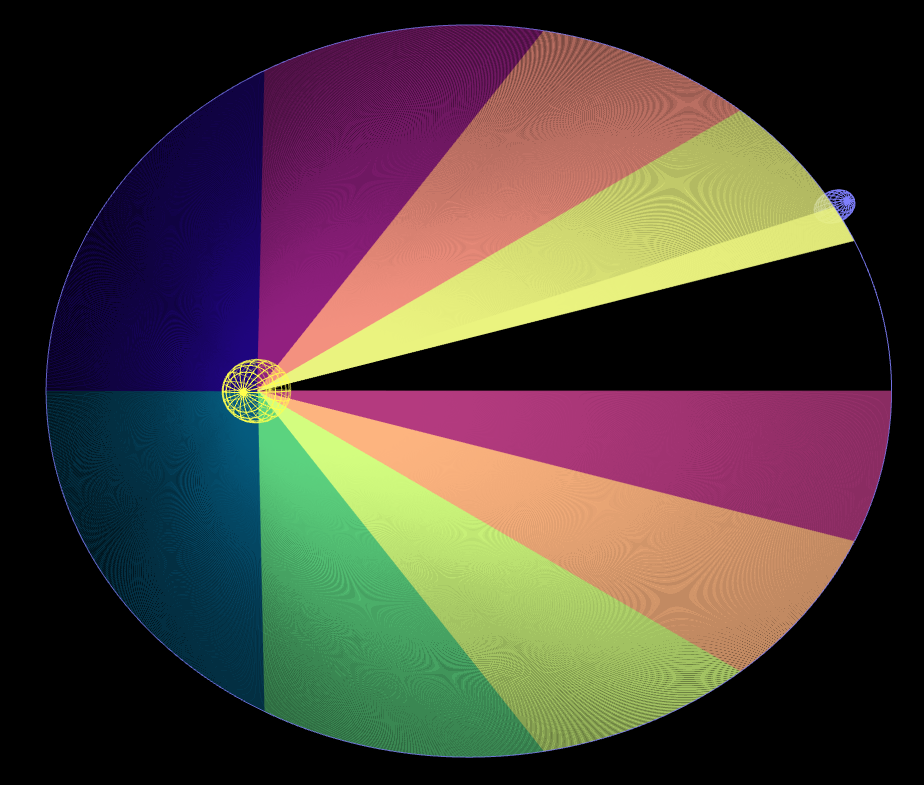
\includegraphics[width=0.5\textwidth]{equal-areas.png}

\bigskip
\bigskip

Each colored wedge has the {\it same area}, and the planet takes the {\it same time} to go through each.

\bigskip
\bigskip

This means that it moves {\it faster} when it's nearer the Sun.
\EC
}

\frame{\frametitle{\textbf{Kepler's Third Law}}

\Large
Kepler's third law of orbital motion says that the square of a planet's {\it orbital period} is proportional
to the cube of its {\it semimajor axis}.

\bigskip
\bigskip
\bigskip

Simply put: if a planet is further from the Sun, it takes longer to go around.

\bigskip
\bigskip
\bigskip

If the distance is doubled, the time required {\it more than doubles}.

\bigskip
\bigskip
\bigskip

Let's watch this...

}

\frame{
\Large
Saturn's orbit is about 10 AU across, while Uranus' orbit is about 20 AU across.

\bigskip
\bigskip

Saturn takes about 30 years to orbit the Sun. About how long does Uranus take?

\bigskip
\bigskip

\huge

\color{A}A: About 30 years\\
\color{B}B: Between 30 and 60 years \\ 
\color{C}C: More than 60 years \\
\color{D}D: It depends on the masses of Uranus and Saturn \\
\pause
\color{E}E: I looked it up on Wikipedia...
}

\frame{
\BC
\Huge
Complete {\it Lecture Tutorials} pp. 21-24 (Kepler's second law) and pp. 25-28 (Kepler's third law).
\bigskip
\bigskip

\Large
We will do something else after this (15-20 min)
\EC
}

\frame{\frametitle{\textbf{Do Kepler's laws apply to things other than planets?}}

{\it [They] would also apply to moons orbiting planets, you can confirm this by looking at their orbital patterns. }

\begin{flushright} --Molly\end{flushright}

\BS\pause

{\it No. [They apply] to all celestial objects that orbit a large, massive object. Observe Jupiter and Jupiter's moons, for example.}

\begin{flushright} --Ricky\end{flushright}

\BS\pause


{\it [Kepler's laws only apply to the planets] because the stars do not orbit the Sun. The fact that they appear to stay in the same spot confirms my conclusion.}

\begin{flushright} --Caitlin\end{flushright}

\BS\pause

{\it No. Think about the earth and the moon. Moon is orbiting around the earth, and Kepler's laws should also apply [to the] moon's orbiting.}

\begin{flushright} --Jiaqi\end{flushright}

}
\frame{\frametitle{\textbf{Are Kepler's laws of orbital motion fundamental laws of Nature}}

{\it Considering Kepler's laws of orbital motion as fundamental laws of Nature is correct- gravity itself is what causes "nature", same as physics. Without gravity, which is what causes such orbital motion, the Earth itself would have never formed, gravity is "nature" itself.}

\begin{flushright} --Snider\end{flushright}

\BS\pause

{\it Not necessarily, I [think] laws of Nature should refer to a law or principle that is applicable to a lot of things in nature. Kepler's laws are only applicable to planets, stars and comets. I think what would be more fundamental at play here is gravity or even the concept of the ellipse occurring in nature. }

\begin{flushright} --Lilyann\end{flushright}

\BS\pause

{\it Kepler's laws are a result of gravity, which is the "something more fundamental".} 

\begin{flushright} --Noa\end{flushright}

\BS\pause


{\it [There is a] more fundamental thing that cause[s] them. In my opinion, we [see] the planets that orbit this way because of the gravity from star[s]. The gravity of stars attracts the planet and Kepler's laws explain the result of gravity in a mathematical way.} 

\begin{flushright} --Yuxin\end{flushright}

\BS\pause

}
\frame{\frametitle{\textbf{Where are we now?}}
\Large

Kepler figured out what had eluded everyone else: a precise description of the orbits of the planets.

\bigskip
\bigskip
\bigskip

\pause

But he thought there was more: that the planets' orbits were {\it caused} by the interplay of more fundamental agents.

\bigskip
\bigskip
\bigskip

He didn't have a good name for them: we now call them ``gravity'' and ``inertia''. We'll learn about those soon.
}

\frame{\frametitle{\textbf{Natural laws vs. their consequences}}
\Large
Obviously the world around us is very diverse. Some things in it look quite simple:

\BI
\item{The motion of the stars}
\item{The near-perfect-spheres of the planets and moons}
\item{The elliptical motions of the planets (?)}
\item{The colors in a rainbow}
\EI
\pause
\bigskip

Others, though, are maddeningly complex:

\BI
\item{Seismic waves and earthquakes}
\item{The colors in the Sun}
\item{The weather}
\item{The diversity of rocks on Earth}
\pause
\item{Even the simplest living things}
\pause
\item{... language, culture, music, art, and all the creations of humankind...}
\EI
}

\frame{\frametitle{\textbf{Elegance, revisited}}

\BC
\Large

The laws of the Universe are simple and elegant. 

The things the Universe builds out of them are often complex!

\bigskip
\bigskip
\bigskip
\EC
\begin{columns}
\column{0.5\textwidth}
\BC
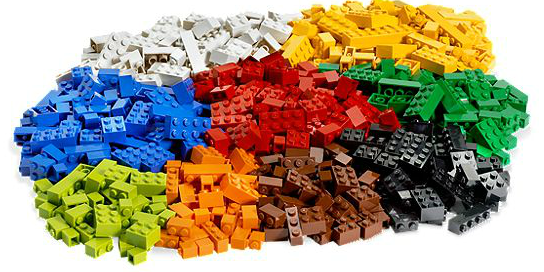
\includegraphics[width=0.8\textwidth]{lego-set.png}
\EC
\pause
\column{0.5\textwidth}
\BC
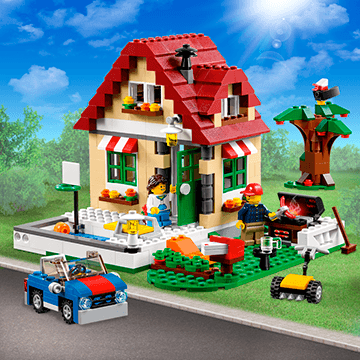
\includegraphics[width=0.8\textwidth]{lego-house.png}
\EC
\end{columns}
}



%\frame{\frametitle{\textbf{Natural laws vs. their consequences}}
%\large
%We've been doing science for a few hundred years, and we've noticed a pattern.
%
%\bigskip
%
%The Universe seems to operate according to a {\it very few} basic laws.
%\BI
%\item{There are {\it four forces} in nature, two of which are different manifestations of the same thing}
%\item{All these forces cause a few types of {\it elementary particles} to move around}
%\item{On a very small scale, this movement is governed by the laws of {\it quantum mechanics}}
%\item{On a bigger scale, QM turns into the much simpler {\it Newton's laws of motion}}
%\item{This movement takes place on the stage of {\it spacetime}}
%\EI
%
%\pause
%
%\bigskip
%
%When things are complicated (not simple and elegant) in Nature, it's because they are {\it complicated combinations} of pieces that are, themselves, simple -- pieces that obey simple laws.
%
%\pause
%\bigskip
%\bigskip
%
%... even us!
%}

\frame{\frametitle{\textbf{Isaac Newton}}

\begin{columns}
\column{0.4\textwidth}
\BC
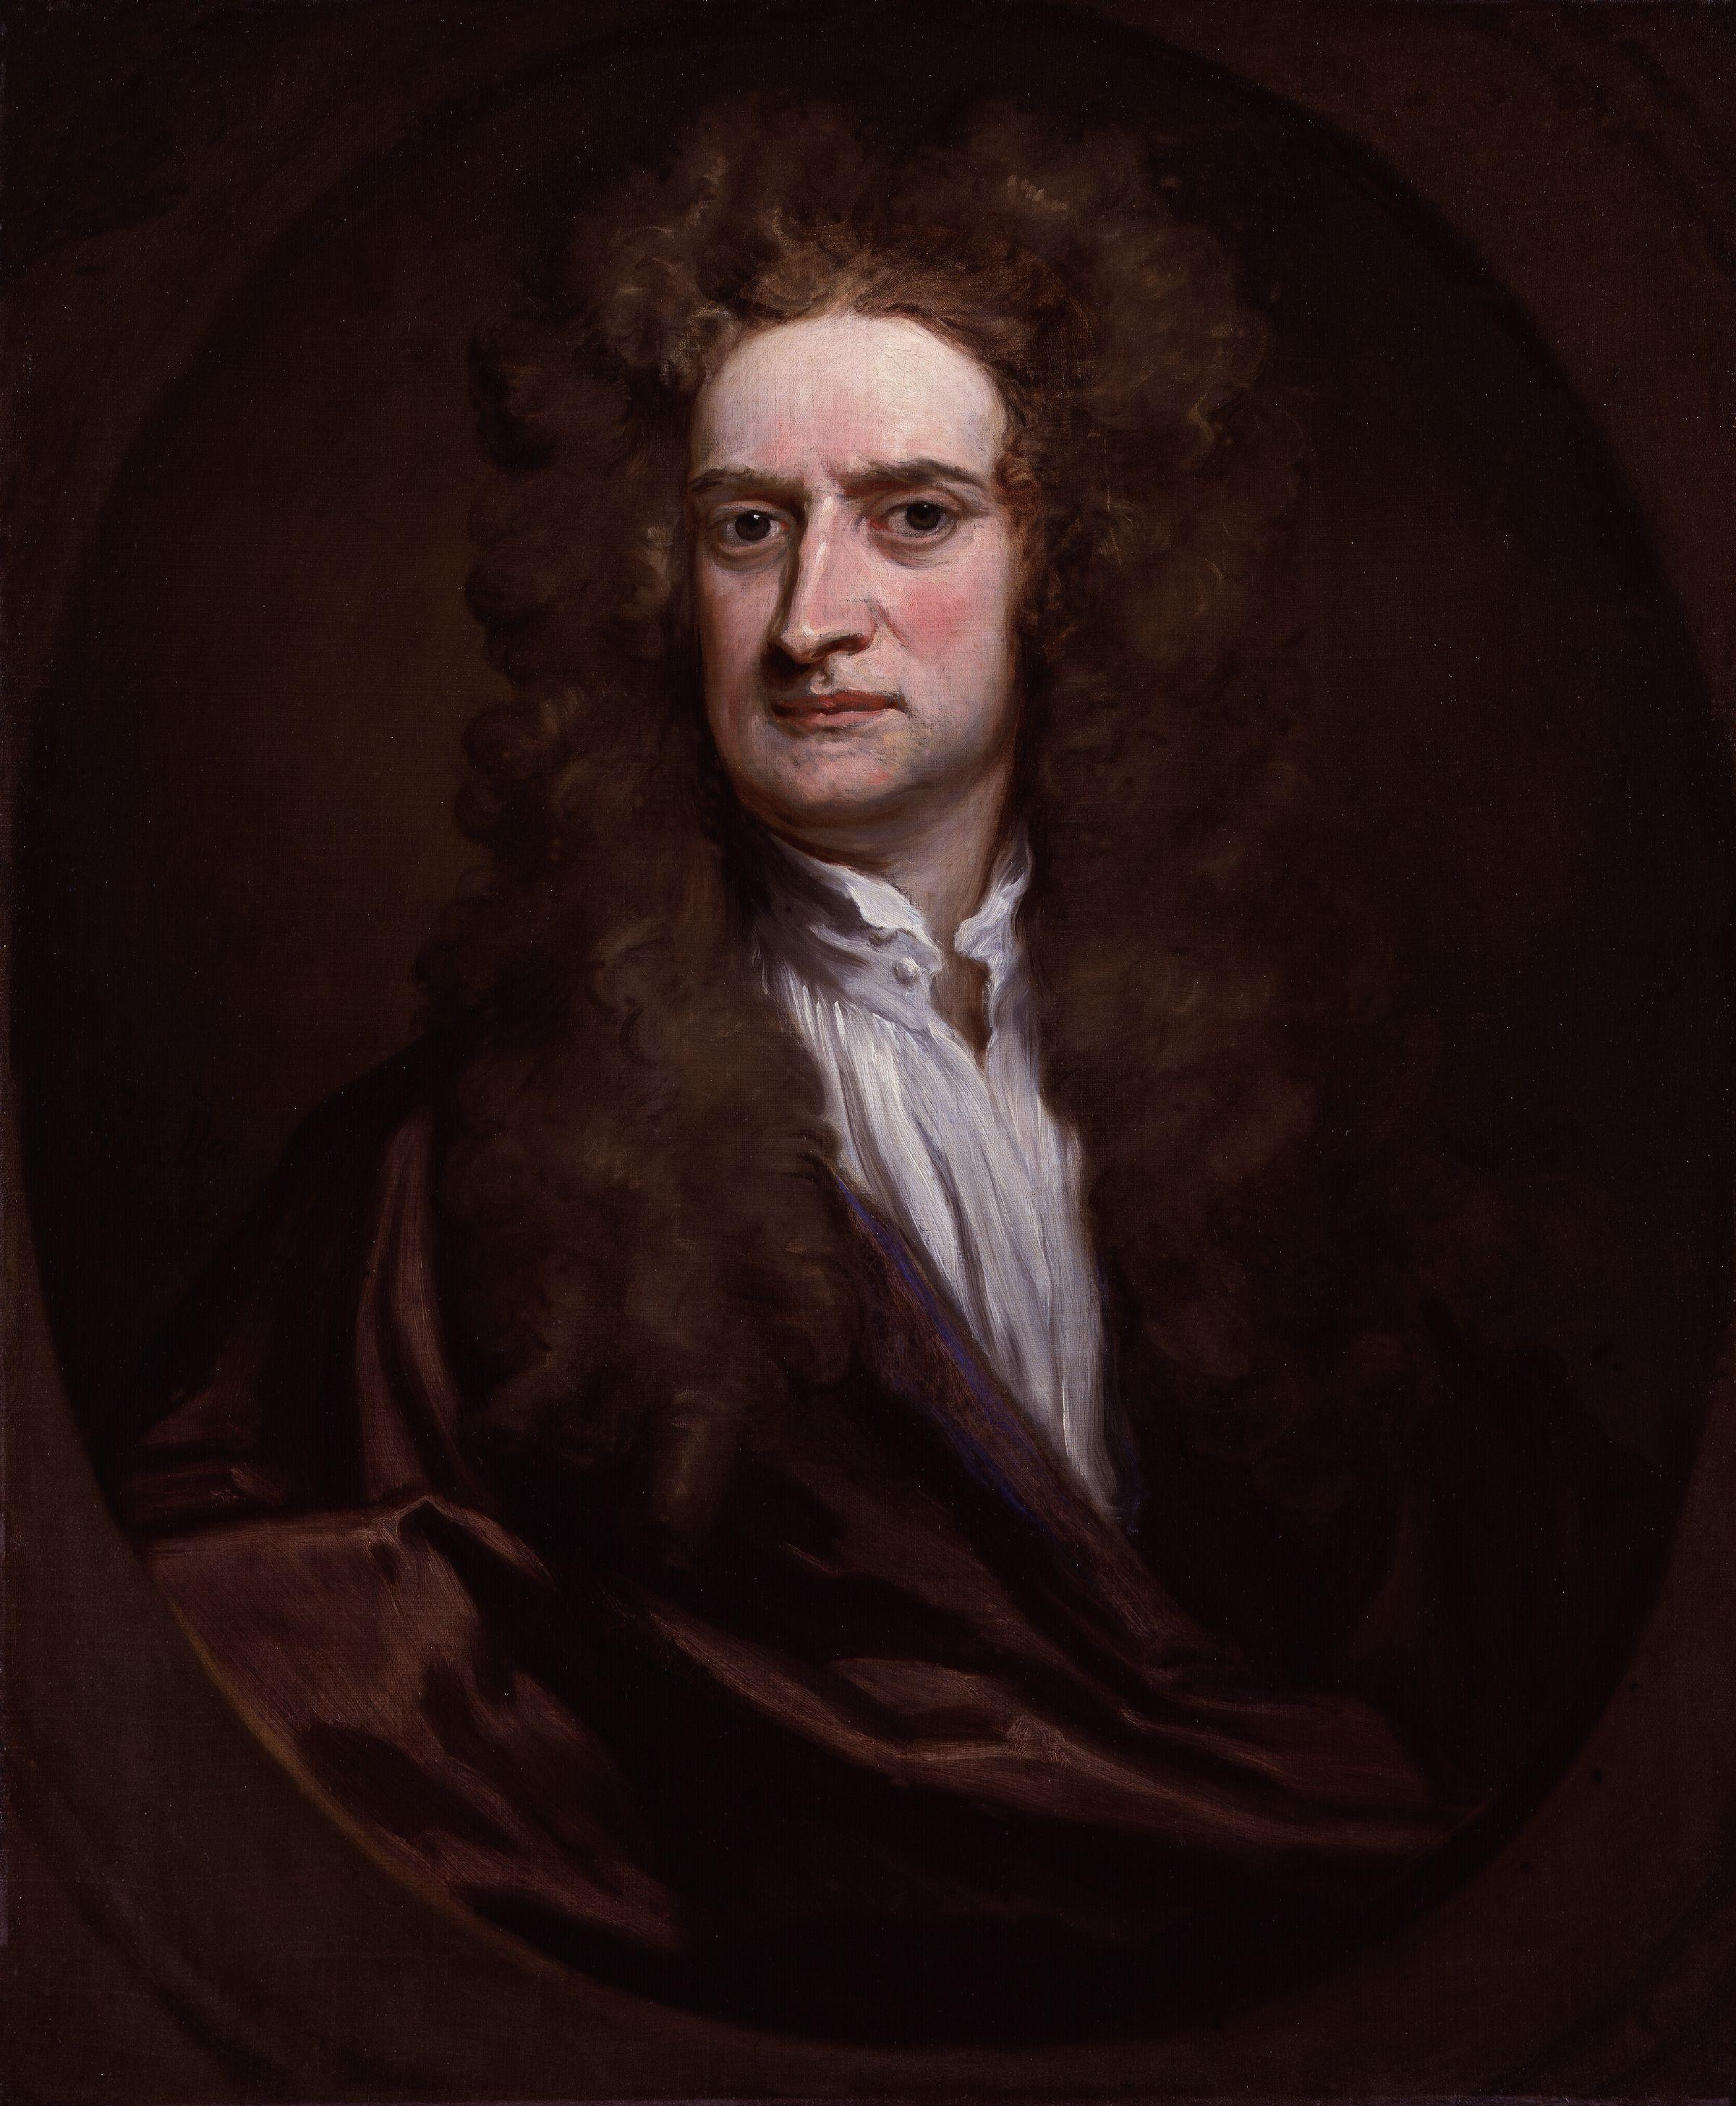
\includegraphics[width=\textwidth]{newton.jpg}
\EC
\column{0.6\textwidth}

\large
Isaac Newton (1642-1727 or 1726) finally figured out the laws that eluded Kepler.

\bigskip

He discovered...

\BI
\item{Forces cause objects to change their speed or direction of motion}
\item{Calculus -- the mathematics of changes}
\item{Gravity is such a force}
\item{The mathematical description of gravity}
\pause
\item{Principles of optics}
\item{The mathematics of cooling}
\item{... and much more}
\EI
\end{columns}
}


\frame{\frametitle{\textbf{Newton's biggest idea}}

\Huge
\BC

``Forces cause objects to accelerate''

\bigskip
\bigskip
\bigskip

$F=ma$

\bigskip
\bigskip
\bigskip

$F/m = a$

\bigskip
\bigskip
\bigskip

\Large

``The strength of a force, divided by the mass of the thing it acts on, gives that thing's acceleration''
\EC
}

\frame{\frametitle{\textbf{The law of gravity}}
\Large
Newton showed mathematically what Kepler suspected. 

\bigskip
\bigskip

All objects attract all other objects with a force that is:

\BI
\item{Proportional to the product of their masses}
\item{Inversely proportional to the distance between them squared}
\EI

In symbols:

$$F = \frac{G m_1 m_2}{r^2}$$
}

\frame{
\Large
Suppose two asteroids are floating out in space. Asteroid A is twice as massive as asteroid B.

\bigskip

If the force of A's gravity on B is ten tons, the force of B's gravity on A will be...

\huge

\bigskip

\color{A}A: 5 tons\\
\color{B}B: 10 tons\\
\color{C}C: 20 tons\\
\color{D}D: 40 tons
}

\frame{\frametitle{\textbf{The law of gravity}}
\Large

All objects attract all other objects with a force that is:

\BI
\item{Proportional to the product of their masses}
\item{Inversely proportional to the distance between them squared}
\EI

In symbols:

$$F = \frac{G m_1 m_2}{r^2}$$

\BC
\color{Red}
Notice I didn't say which mass was which. It doesn't matter!
\EC

}

\frame{
\Large
Suppose two asteroids are floating out in space, 20 miles apart. Asteroid A is twice as massive as asteroid B,
and the force of A's gravity on B is ten tons.

\bigskip

Suppose I now move the two asteroids closer, so they're only 10 miles apart. What will the force of A's gravity on B be now?

\huge

\bigskip

\color{A}A: 5 tons\\
\color{B}B: 10 tons\\
\color{C}C: 20 tons\\
\color{D}D: 40 tons
}



\end{document}
